\section{Introduction}

    Many programs fall victim to having lots of redundant code.
    Right from simple redundant writes to outright dead code, removing them plays a major role in performance of our programs. 
    Such redundancy could also be possible due to different phases of optimization the compiler performs, which leaves certain residual code in each phase.
    Examples of such optimizations are common-sub-expression elimination, copy propagation, partial redundancy elimination, register allocation, etc.
    
    In a sequential setting the effect of removing such code is expected to be invisible to execution.    
    However, as we saw for instruction reordering, in a concurrent setting, elimination may not be that straightforward. 
    
    \paragraph{Write Elimination}
    
        Consider the first example in Figure~\ref{elim:example1(a)} below of a Candidate (left) and the resultant candidate after eliminating a write (right).
        The orange box shows the observable behavior that we want to consider. 
        Note that here, the outcome of read values of $b$ and $c$ are not relevant for our purpose. Hence they can have any value.
        \begin{figure}[H]
            \centering
            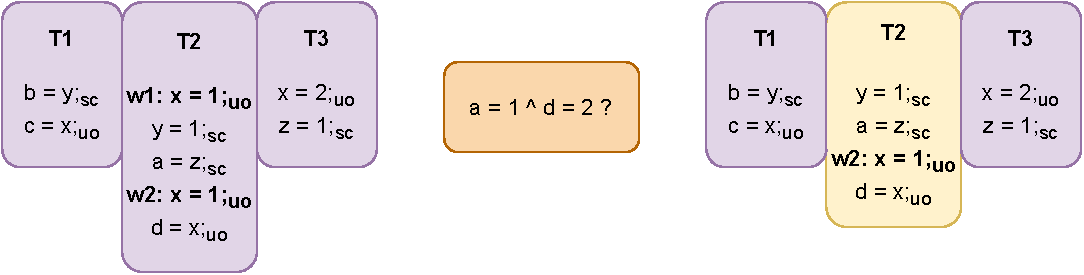
\includegraphics[scale=0.7]{5.Elimination/EliminationExample1(a).pdf}
            \caption{First example for elimination with candidates of the original program and its counterpart after elimination of a write.} 
            \label{elim:example1(a)}
        \end{figure}

        Figure~\ref{elim:example1(b)} explains the relations implied in a candidate execution based on Observable behaviors that disallows the behavior in question (top) for the original program but is valid for that after elimination (below). 

       The first set of relations is for the original program, where Axiom \ref{CoRe} prohibits the read $d$ to have value of $x$ as $2$.
        For $a$ to have value $1$, it must come from the write $z=1;_{sc}$.
        From this we can infer $\reln{\{z=1;_{sc}\}}{hb}{\{a=z;_{sc}\}}$.
        From Def of agent order and happens-before, we can infer $\reln{\{x=2;_{uo}\}}{hb}{\reln{\{w2:x=1;_{uo}\}}{hb}{\{d=x;_{uo}\}}}$.
        By Axiom \ref{CoRe}, the read value of $d$ cannot be $2$. 
    
        The second set is for the modified program, where none of the axioms restrict such a behavior (I would suggest the avid readers to check it for themselves).
        For $a$ to have value $1$, it must come from the write $z=1;_{sc}$.
        From this we can infer $\reln{\{z=1;_{sc}\}}{hb}{\{a=z;_{sc}\}}$.
        From Def of agent order and happens-before, we can infer $\reln{\{x=2;_{uo}\}}{hb}{\{d=x;_{uo}\}}$.
        The above relations do not restrict $d$ from having value $2$.
    
        \begin{figure}[H]
            \centering
            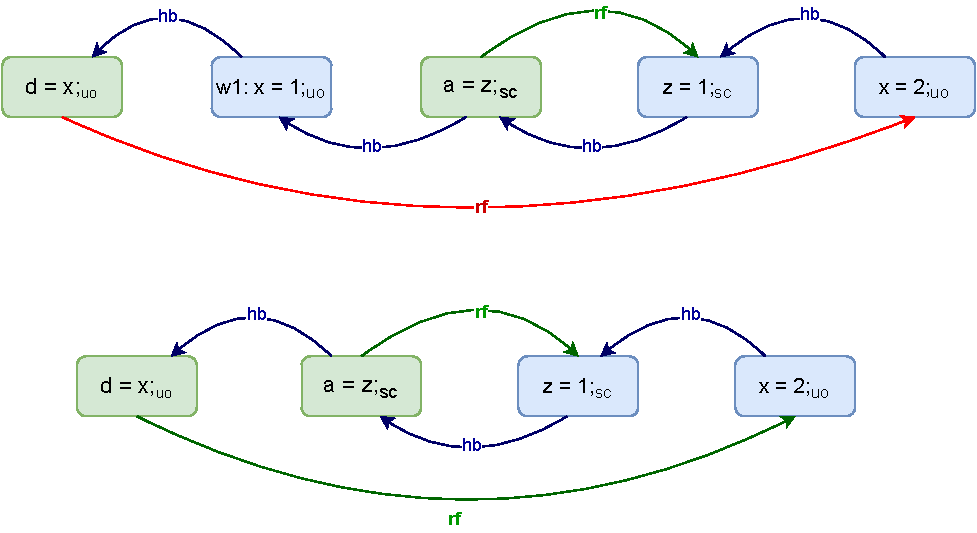
\includegraphics[scale=0.7]{5.Elimination/EliminationExample1(b).pdf}
            \caption{The set of partial order relations justifying whether the observable behavior in question is allowed for both the candidates in Figure~\ref{elim:example1(a)}. Note that the red arrow of $\stck{_{rf}}$ signifies a relation that is not allowed.} 
            \label{elim:example1(b)}
        \end{figure}

        In the same above example, if the compiler decides to eliminate $w1$, then the observable behavior $b=1 ^ c=0$ will be allowed (we leave it as an exercise for the reader to verify).
        This is a classic example of where, a sequentially sane optimization by elimination is not possible, whatever the choice of write we choose to eliminate.  

    \paragraph{Read Elimination}
    
        In the case of read elimination, we clearly would lose observable behaviors w.r.t. to the read eliminated.
        However, our focus is more on whether eliminating this read introduces new observable behaviors in the remaining program, meaning, can other reads be affected.
        Constructing such an example is non-trivial and involves implied memory order edges that are created between events.
        Figure~\ref{elim:example2(a)} shows such an example where the Original Candidate (left) and the one after eliminating a read in $T2$ is shown.
        The orange box represents the behavior in question. 
        \begin{figure}[H]
            \centering
            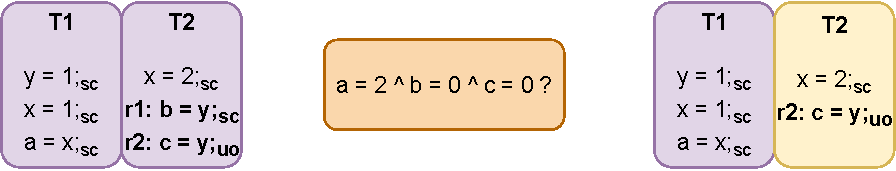
\includegraphics[scale=0.7]{5.Elimination/EliminationExample2(a).pdf}
            \caption{First example for elimination with candidates of the original program and its counterpart after elimination of a read.} 
            \label{elim:example2(a)}
        \end{figure}

        Figure~\ref{elim:example2(b)} explains the relations formed in a candidate execution that disallow the behavior in question for the original program but justify it after elimination. 

        The first set of relations are for the original program, where the outcome in question is not allowed.
        For $a$ to have value $2$, it must come from the write $x=2;_{sc}$.
        From this, we can imply $\reln{\{x=2;_{sc}\}}{hb}{\{a=x;_{sc}\}}$.
        From Def of agent order, we can imply $\reln{\{x=1;_{sc}\}}{hb}{\{a=x;_{sc}\}}$.
        From the above relations, we can imply the memory order $\reln{\{x=1;_{sc}\}}{mo}{\{x=2;_{sc}\}}$ (note that if the memory order was reversed, Axiom \ref{SeqCsAt} would disallow the read value of $a$ to be $2$).
        By Def of memory order, we can now imply $\reln{\{y=1;_{sc}\}}{mo}{\{b=y;_{sc}\}}$.
        We already have by Def of happens-before that $\reln{\{y=0;_{init}\}}{hb}{\{b=y;_{sc}\}}$ and $\reln{\{y=0;_{init}\}}{hb}{\{y=1;_{sc}\}}$.
        The above relations, by Axiom \ref{SeqCsAt} prohibits the read $b$ to have value of $y$ as $0$.
        Thus $b$ can only have the value $1$.
        This in turn results in a happens-before relation $\reln{\{y=1;_{sc}\}}{hb}{\{b=y;_{sc}\}}$, which then by Axiom \ref{CoRe} prohibits the read $c$ to have value of $y$ as $0$.
            
        The second set is for the modified program, where none of the axioms restrict such a behavior. 
        We still retain the relations $\reln{\{x=2;_{sc}\}}{hb}{\{a=x;_{sc}\}}$, $\reln{\{x=1;_{sc}\}}{hb}{\{a=x;_{sc}\}}$ and $\reln{\{x=1;_{sc}\}}{mo}{\{x=2;_{sc}\}}$. 
        But now, we have just $\reln{\{y=1;_{sc}\}}{mo}{\{c=y;_{uo}\}}$, $\reln{\{y=0;_{init}\}}{hb}{\{c=y;_{uo}\}}$ and $\reln{\{y=0;_{init}\}}{hb}{\{y=1;_{sc}\}}$.
        The above set of relations, does not restrict the read value of $c$ to be $0$.
        Thus, such an elimination is not sound for this example\footnotemark..
        \begin{figure}[H]
            \centering
            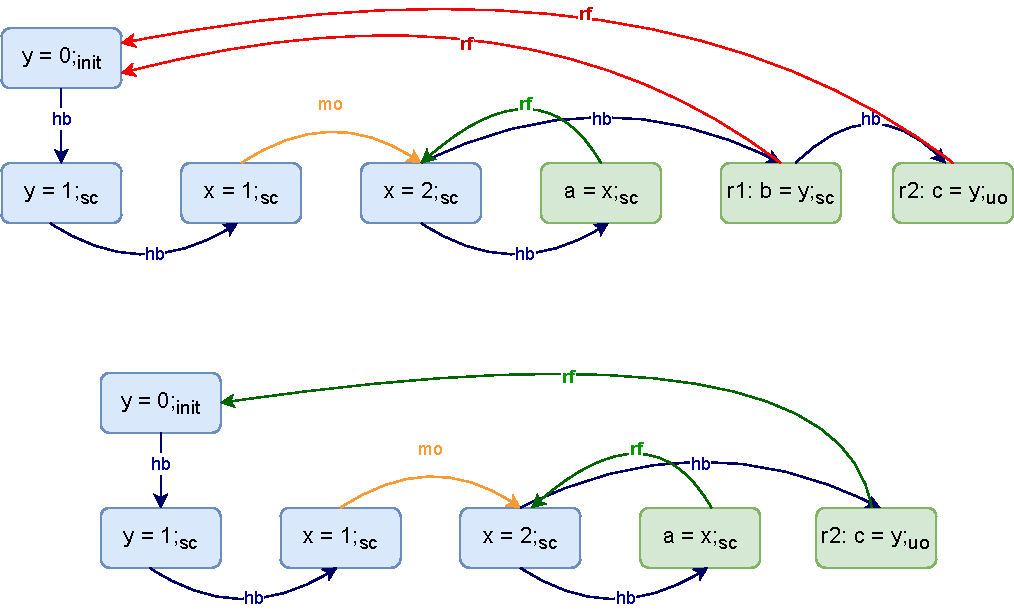
\includegraphics[scale=0.7]{5.Elimination/EliminationExample2(b).pdf}
            \caption{The set of partial order relations justifying the observable behavior in question for both the candidates in Figure~\ref{elim:example2(a)}.} 
            \label{elim:example2(b)}
        \end{figure}
    
        \footnotetext{The avid reader may note that as long as the read value of $a$ is $2$, the value of $c$ can never be $0$. But as we eliminate $b$, none of the axioms disallow the behavior in question.}